\begin{frame}{Datasets}
  \begin{columns}[T]
    \begin{column}{0.38\textwidth}
      {\footnotesize
      \textbf{Paper CSVs (Meghalaya, hourly)}
      \begin{itemize}\setlength\itemsep{0.15em}
        \item \textbf{CPCB}, \textbf{ID1} from Borah et al.
        \item $n \approx 8880$ / $9505$.
        \item NO$_2$, O$_3$, CO, SO$_2$, PM$_{2.5}$, PM$_{10}$.
      \end{itemize}
      \textbf{Extra CAAQMS (15-min $\to$ hourly)}
      \begin{itemize}\setlength\itemsep{0.15em}
        \item \textbf{Shillong:} Lumpyngngad, JN Stadium.
        \item Delhi: ITO, R~K~Puram.
      \end{itemize}
      }
    \end{column}
    \begin{column}{0.60\textwidth}
      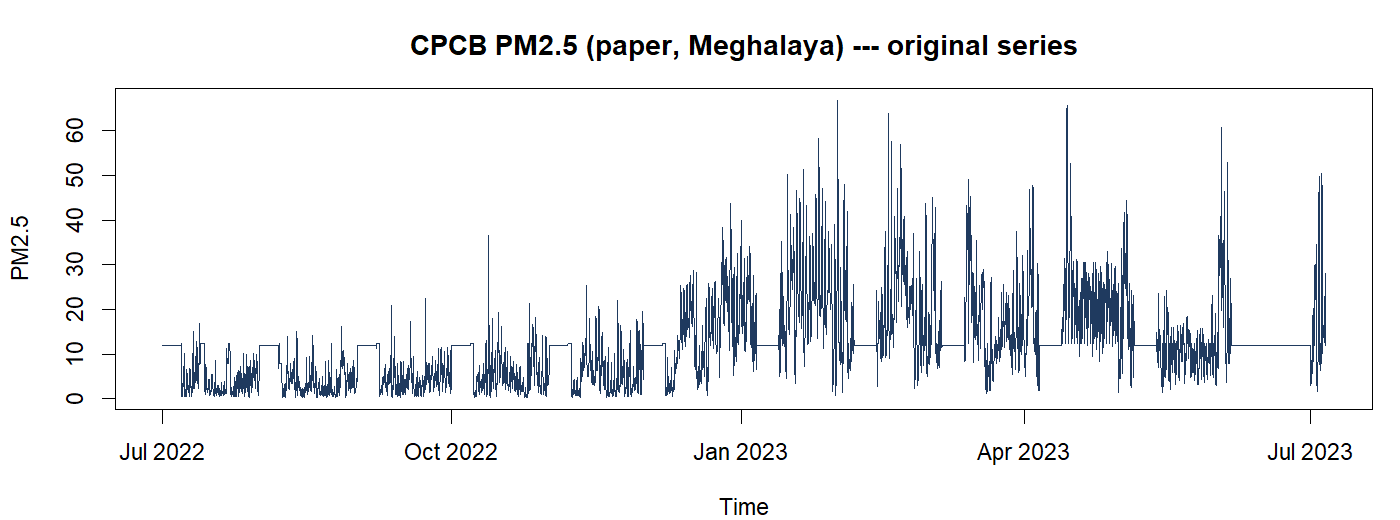
\includegraphics[width=\linewidth]{series_cpcb_pm25.png}\\[-0.2em]
      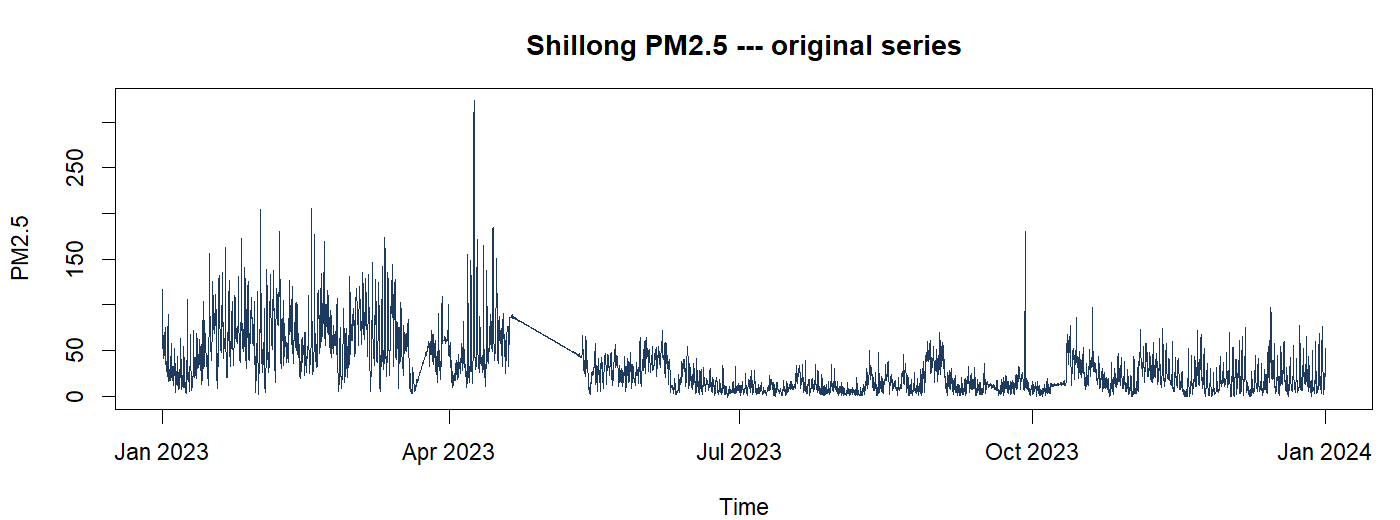
\includegraphics[width=\linewidth]{series_shillong_pm25.png}
    \end{column}
  \end{columns}
\end{frame}

\begin{frame}{Dataset diagnostics --- CPCB PM$_{2.5}$}
  \centering
  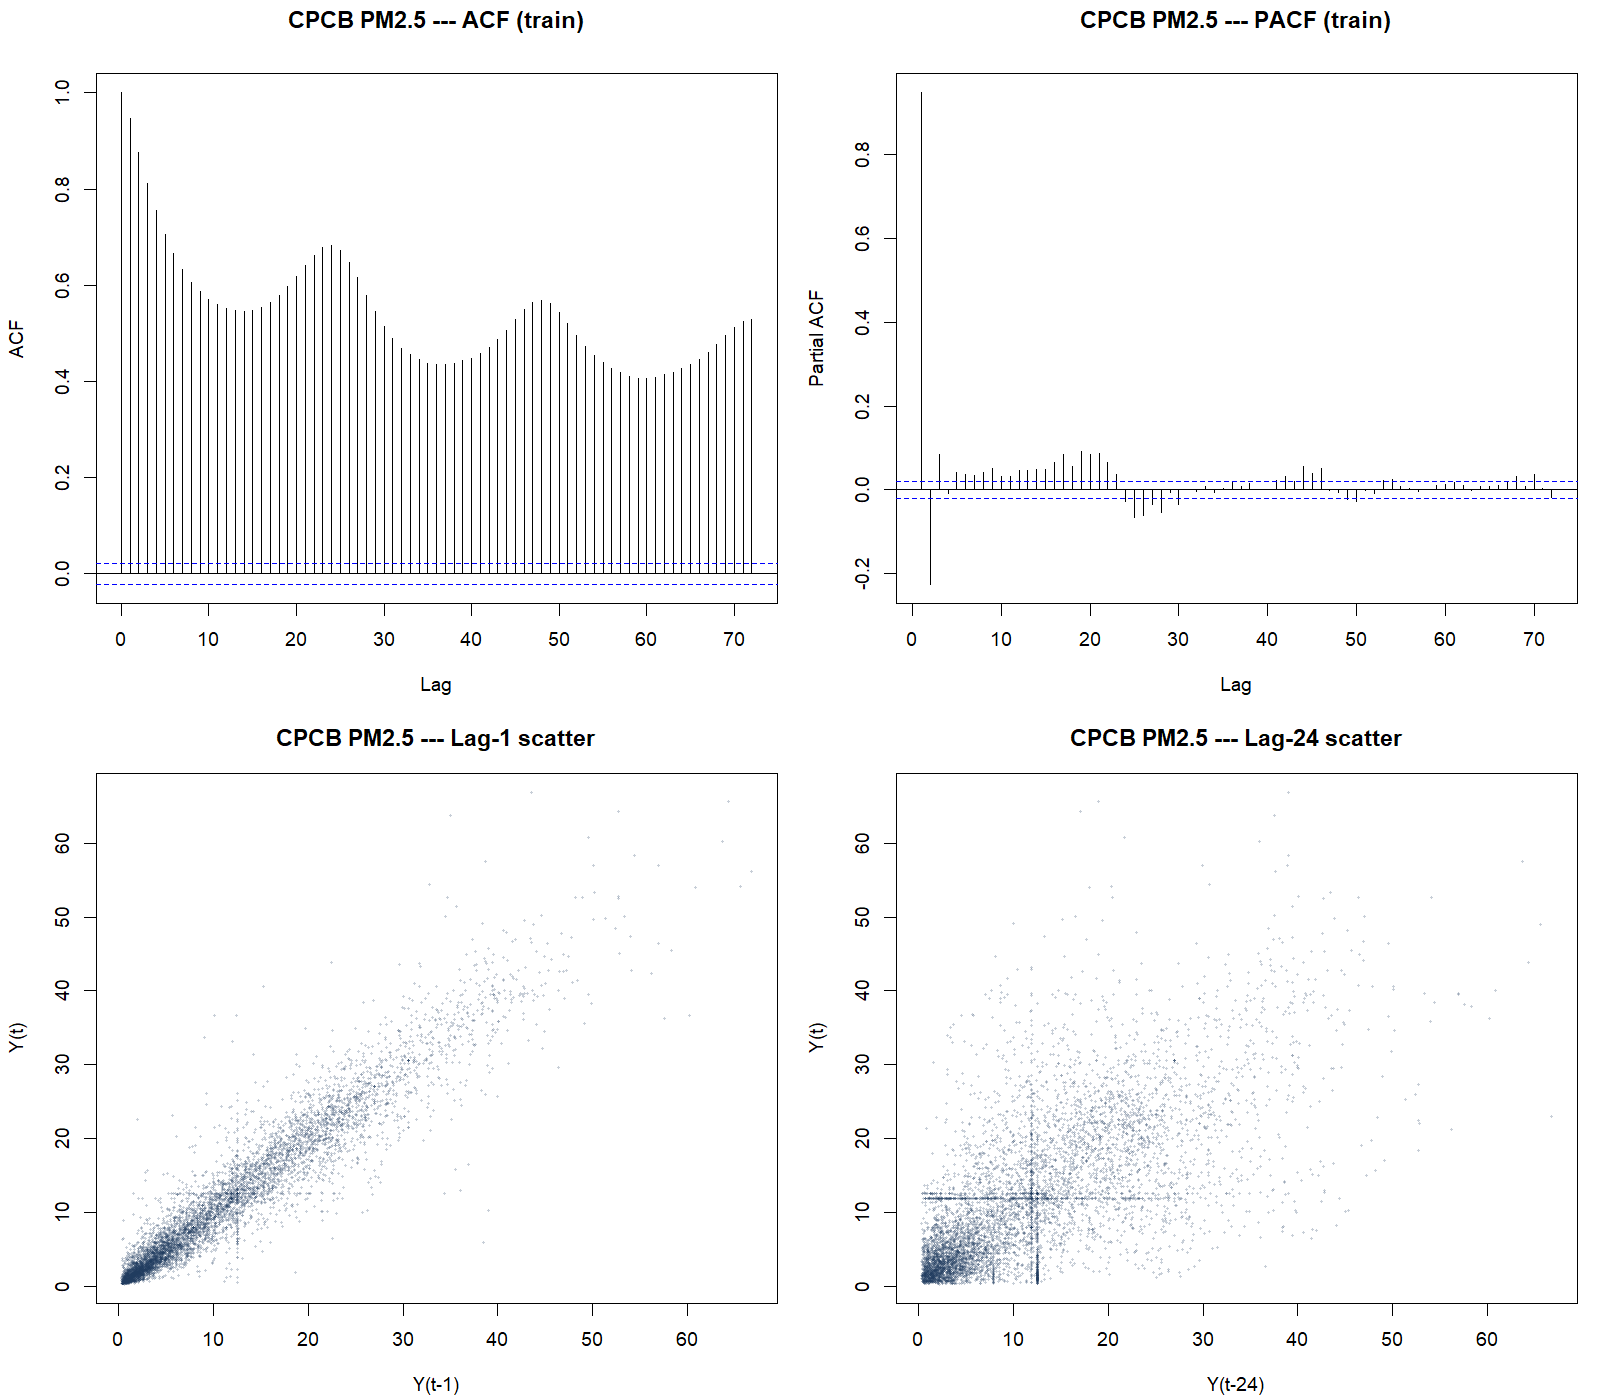
\includegraphics[width=0.98\linewidth,height=0.82\textheight,keepaspectratio]{diag_2x2_cpcb_pm25.png}
\end{frame}

\begin{frame}{Seasonal structure --- CPCB PM$_{2.5}$}
  \centering
  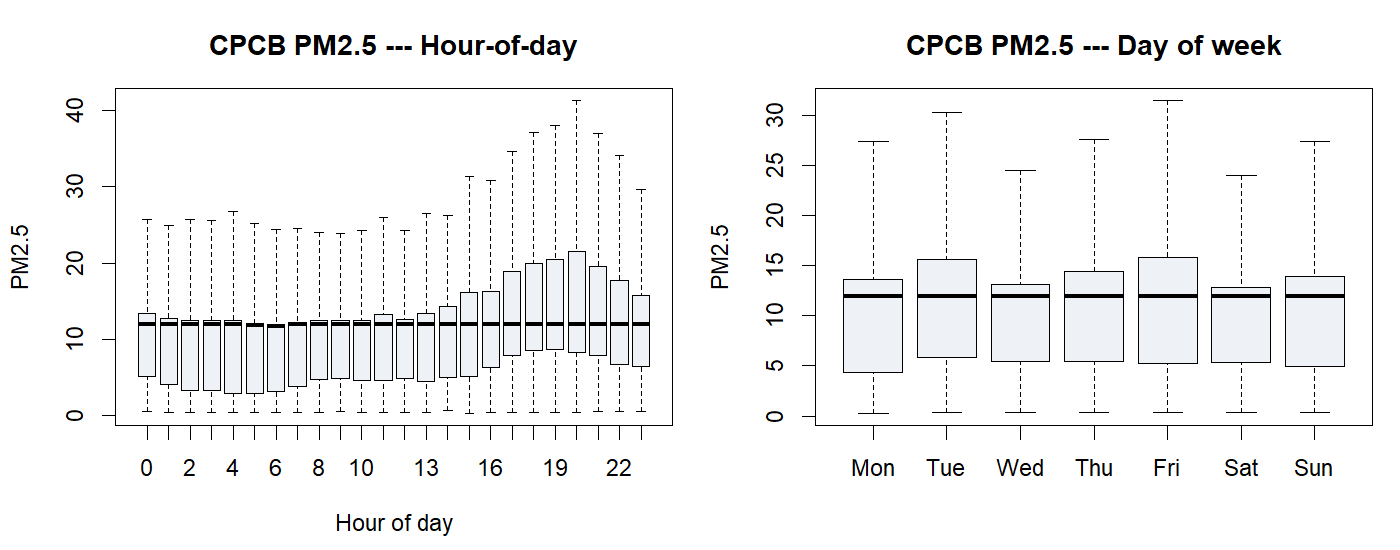
\includegraphics[width=0.95\linewidth,height=0.70\textheight,keepaspectratio]{boxes_cpcb_pm25.png}
  \vspace{0.15em}
  \begin{itemize}
    \item Clear diurnal pattern; milder weekday effect.
    \item Motivates $S=24$ baselines and lag features up to 24~h.
  \end{itemize}
\end{frame}

\begin{frame}{What we did before modelling}
  \begin{itemize}
    \item \textbf{Hourly grid:} end-labelled hourly means (15-min CAAQMS $\to$ hour $t$).
    \item \textbf{Quality screen:} physical bounds, stuck sensors, spike flags.
    \item \textbf{Causal fill:} impute only with information available up to the cut time.
    \item \textbf{Chronological split:} train $\to$ val (tuning) $\to$ test (last $h$ hours).\\
          Horizons $h\in\{24,168,336,744\}$.
    \item \textbf{Scale:} min--max to $[0,1]$ fit on \textbf{train only}.
    \item Paper Meghalaya CSVs are already hourly $\Rightarrow$ skip re-aggregation / fill.\\
          Extra stations (Shillong, Delhi) get the full clean path into an isolated store.
  \end{itemize}
\end{frame}
